\chapter{Bundle Adjustment}
\label{ch:bundle_adjustment}

\section{Overview}

\newenvironment{myindentpar}[1]
               {\begin{list}{}
                   {\setlength{\leftmargin}{#1}}
                 \item[]
               }
               {\end{list}}

\definecolor{lgray}{gray}{0.95}

Satellite position and orientation errors have a direct effect on the
accuracy of digital elevation models produced by the Stereo Pipeline.
If they are not corrected, these uncertainties will result in
systematic errors in the overall position and slope of the \ac{DEM}.
Severe distortions can occur as well, resulting in twisted or ``taco
shaped'' \acp{DEM}, though in most cases these effects are quite
subtle and hard to detect. In the worst case, such as with old mission
data like Voyager or Apollo, these gross camera misalignments can
inhibit Stereo Pipeline's internal interest point matcher and block
auto search range detection.
\begin{figure}[bt]
  \centering
  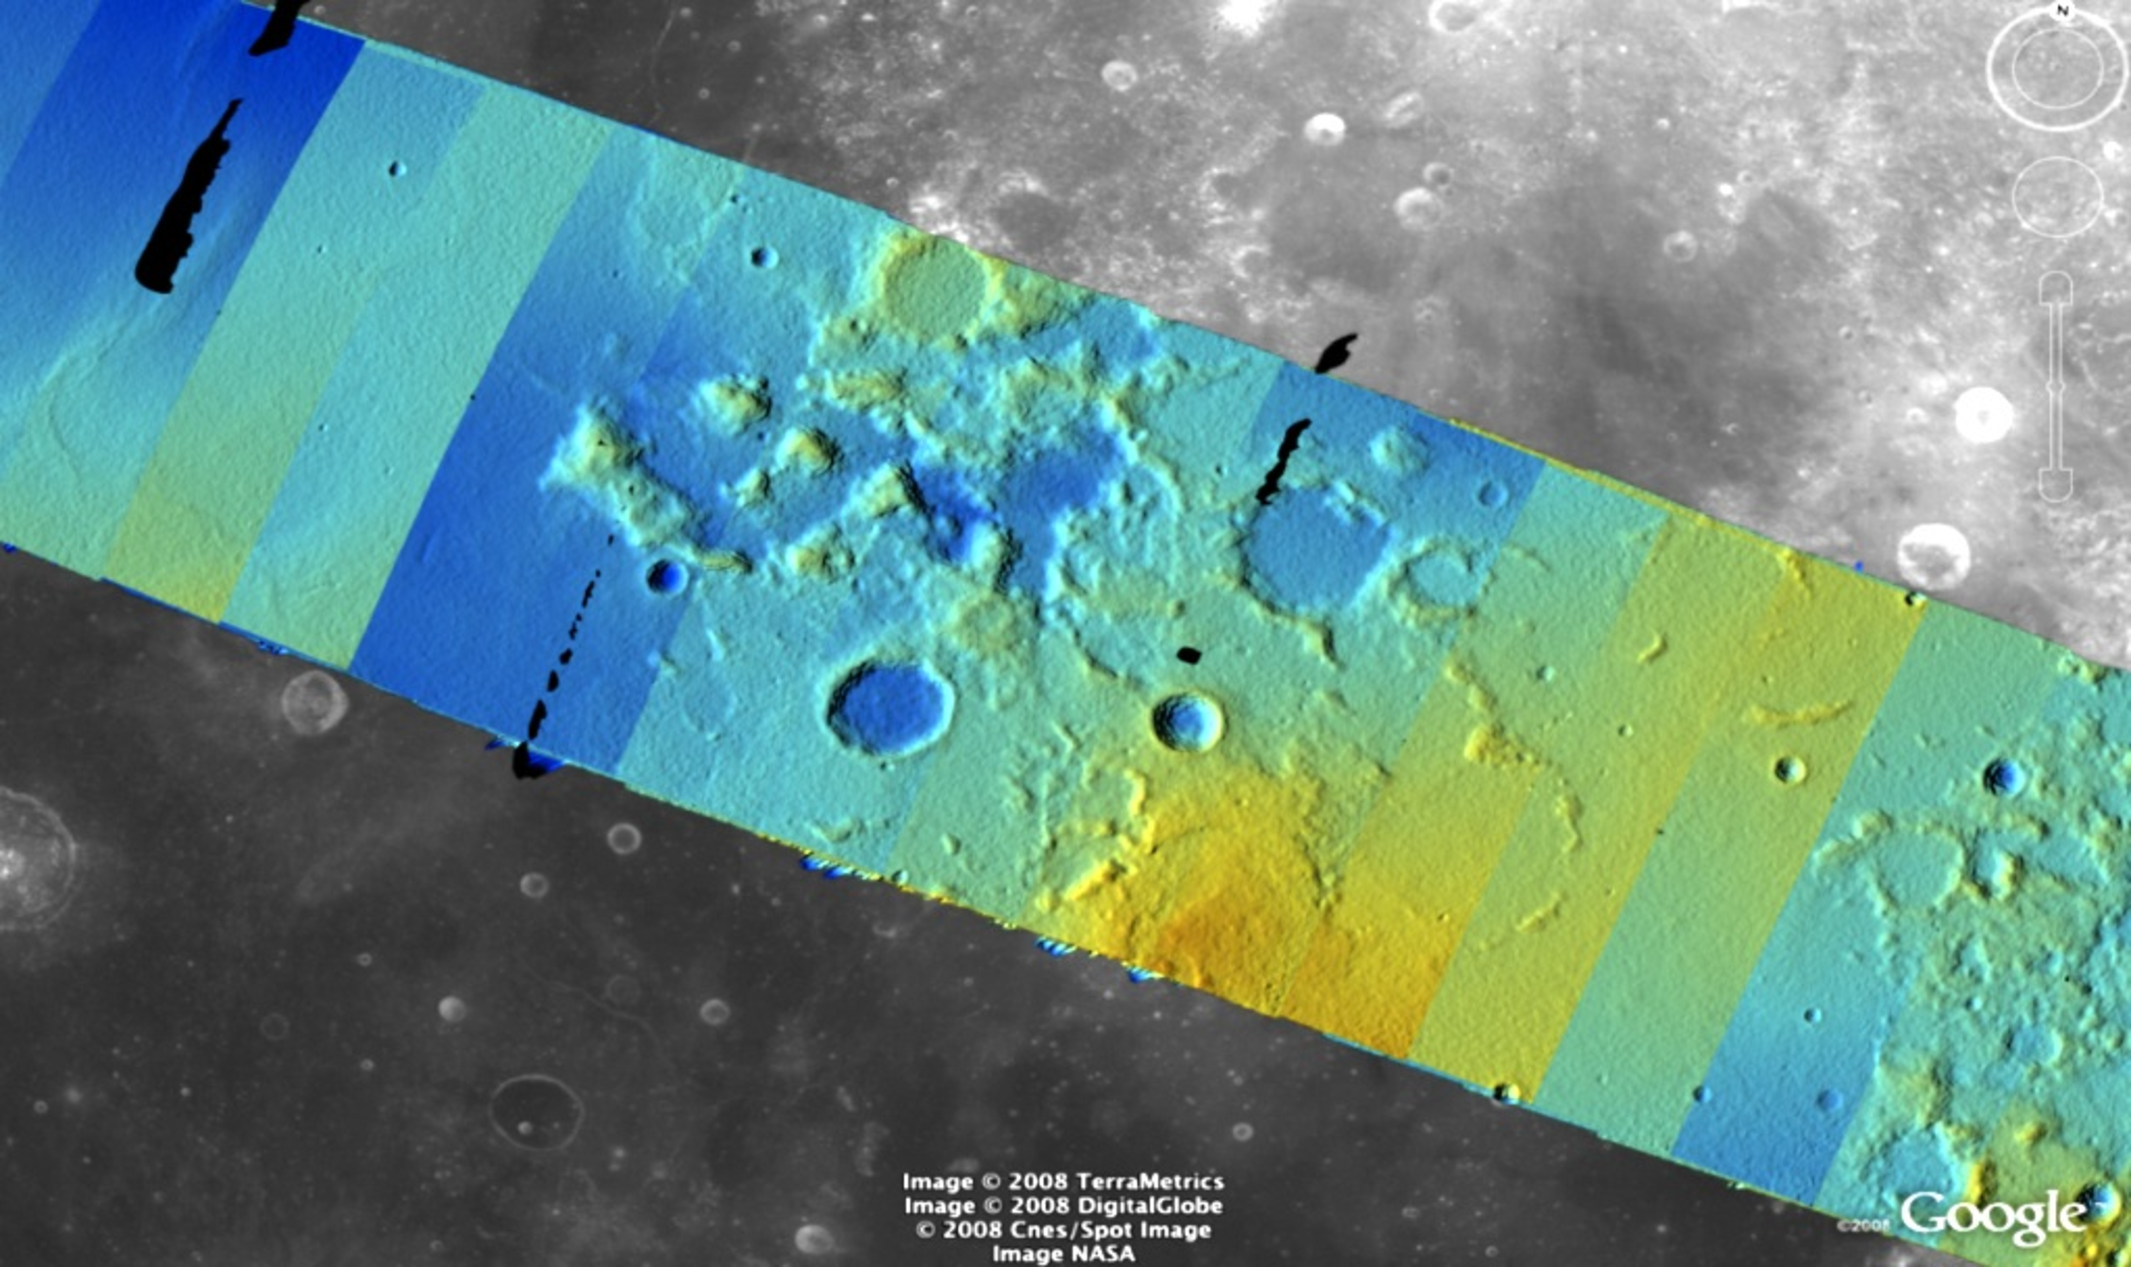
\includegraphics[width=8cm]{images/ba_orig.pdf}
  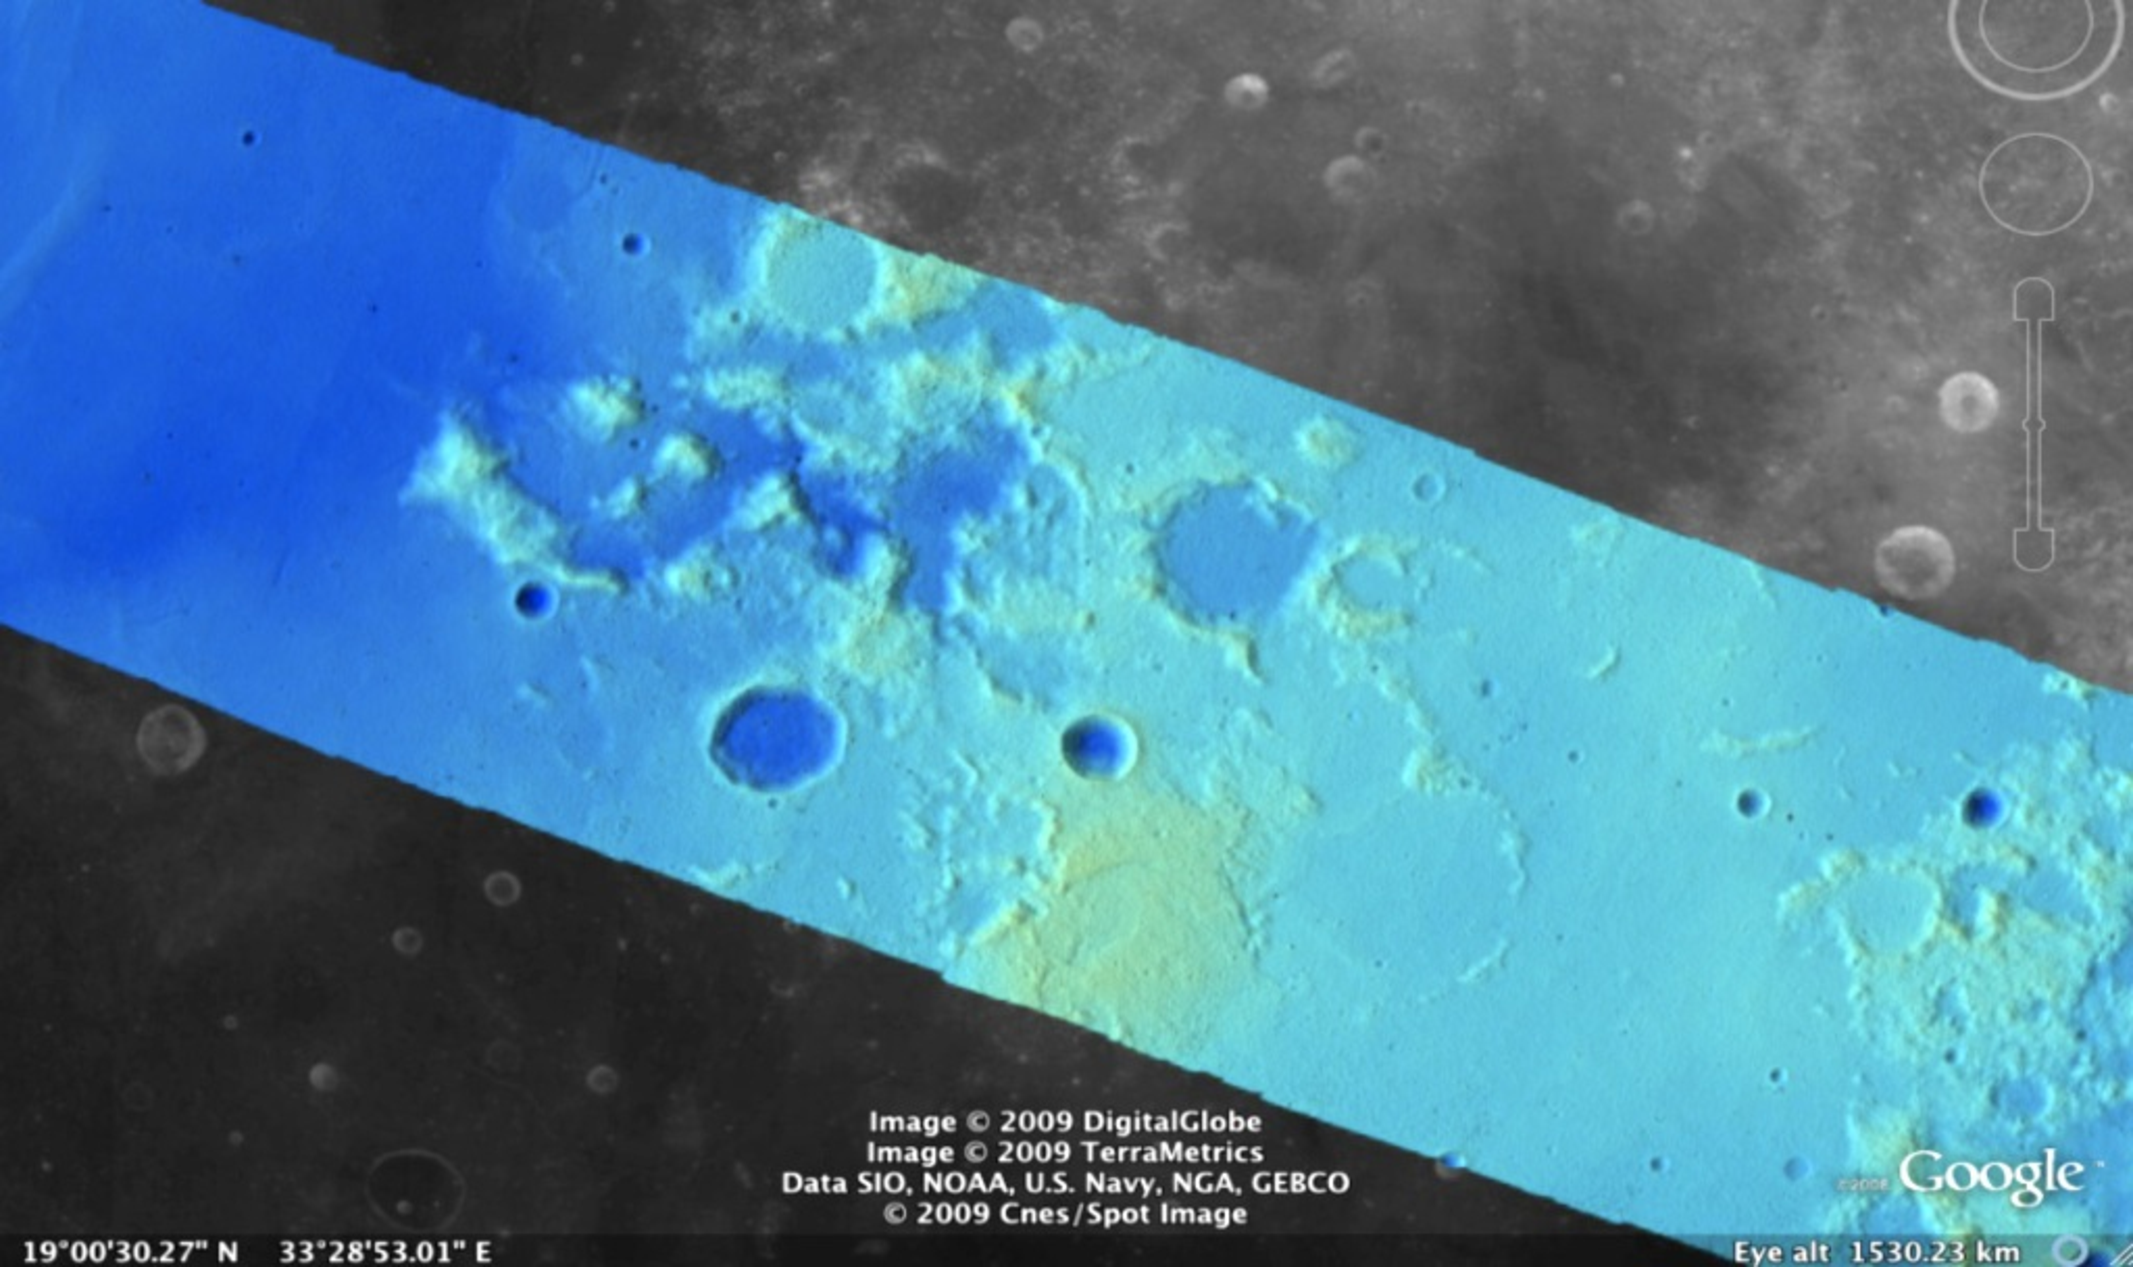
\includegraphics[width=8cm]{images/ba_adjusted.pdf}
  \caption{Bundle adjustment is illustrated here using a color-mapped,
    hill-shaded DEM mosaic from Apollo 15, Orbit 33, imagery. (a)
    Prior to bundle adjustment, large discontinuities can exist between
    overlapping DEMs made from different images. (b) After bundle
    adjustment, DEM alignment errors are minimized and no longer visible.}
  \label{fig:bundle_adjustment}
\end{figure}

Errors in camera position and orientation can be corrected using a
process called \emph{bundle adjustment}. Bundle adjustment is the
process of simultaneously adjusting the properties of many cameras and
the 3D locations of the objects they see in order to minimize the error
between the estimated, back-projected pixel locations of the 3D objects
and their actual measured locations in the captured images.

This complex process can be boiled down to this simple idea: bundle
adjustment ensures that the observations in multiple images of a
single ground feature are self-consistent. If they are not consistent,
then the position and orientation of the cameras as well as the 3D
position of the feature must be adjusted until they are.  This
optimization is carried out along with thousands (or more) of similar
constraints involving many different features observed in other
images.  Bundle adjustment is very powerful and versatile: it can
operate on just two overlapping images, or on thousands. It is also a
dangerous tool. Careful consideration is required to insure and
verify that the solution does represent reality.

Bundle adjustment can also take advantage of \acp{GCP}, which are
3D locations of features that are known a priori (often by measuring
them by hand in another existing \ac{DEM}). \acp{GCP} can improve the internal
consistency of your \ac{DEM} or align your \ac{DEM} to an existing data
product. Finally, even though bundle adjustment calculates the
locations of the 3D objects it views, only the final properties of
the cameras are recorded for use by the Ames Stereo Pipeline. Those
properties can be loaded into the \texttt{stereo} program which
uses its own method for triangulating 3D feature locations.

When using the Stereo Pipeline, bundle adjustment is an optional step
between the capture of images and the creation of \acp{DEM}. The bundle
adjustment process described below should be completed prior to
running the \texttt{stereo} command.

Although bundle adjustment is not a required step for generating
\acp{DEM}, it is {\em highly recommended} for users who plan to
create \acp{DEM} for scientific analysis and publication.  Incorporating
bundle adjustment into the stereo work flow not only results in
\acp{DEM} that are more internally consistent, it is also the correct
way to co-register your \acp{DEM} with other existing data sets and
geodetic control networks.

At the moment however, Bundle Adjustment does not automatically work
against outside \acp{DEM} from sources such as laser altimeters.
Hand-picked \acp{GCP} are the only way for \ac{ASP} to register to those
types of sources.

\section{Bundle adjustment using ASP}
\label{baasp}

Recently, Stereo Pipeline started providing its own bundle adjustment
tool, named \texttt{bundle\_adjust}. Its usage is described in section
\ref{bundleadjust}.

Here is an example of using this tool on a couple of Apollo 15 images,
and its effect on decreasing the stereo triangulation error.

\begin{figure}[h!]
\centering
  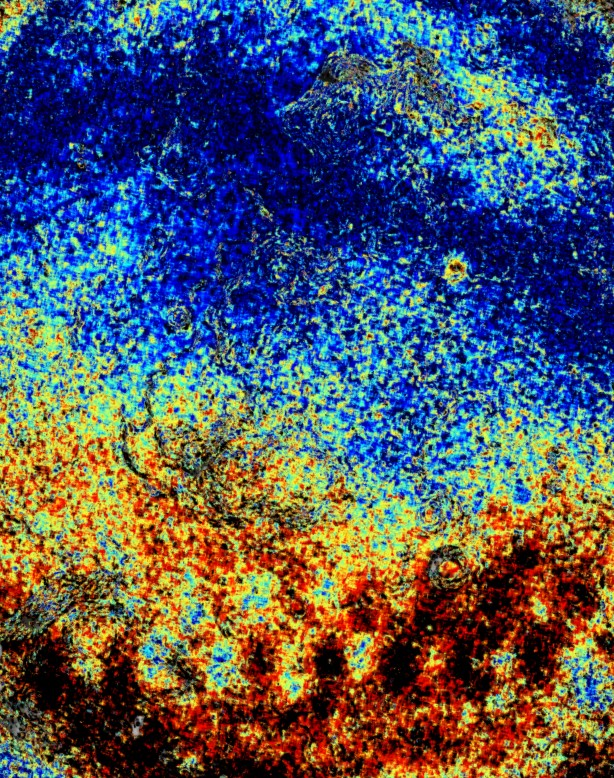
\includegraphics[width=3.0in]{images/examples/before_ba.jpg}
  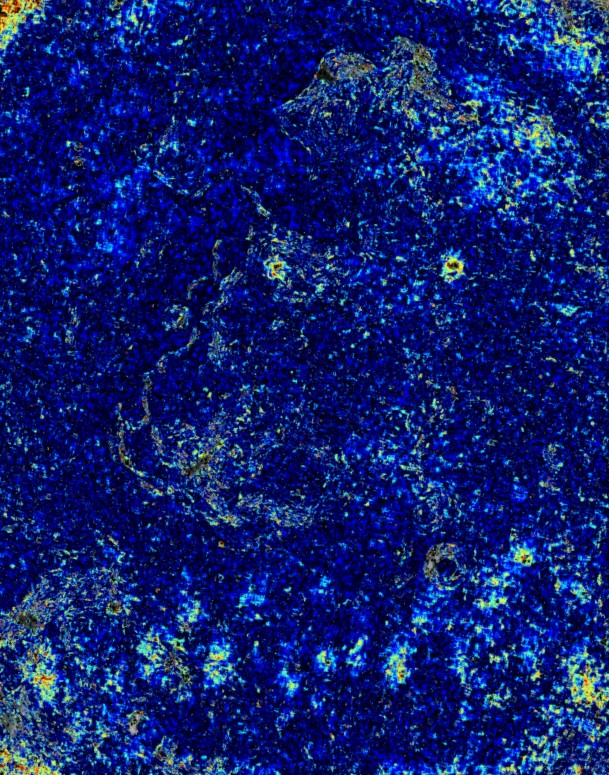
\includegraphics[width=3.0in]{images/examples/after_ba.jpg}
\caption{Illustration of the triangulation error map for a pair of
  images before (left) and after (right) using Stereo Pipeline's
  \texttt{bundle\_adjust}. Red and black colors suggest higher error.}
\label{fig:asp-ba-example}
\end{figure}

Running \texttt{stereo} without using bundle-adjusted camera models.
\begin{verbatim}
  stereo AS15-M-1134.cub AS15-M-1135.cub run_noadjust/run
\end{verbatim}

Performing bundle adjustment.
\begin{verbatim}
  bundle_adjust AS15-M-1134.cub AS15-M-1135.cub -o run_ba/run
\end{verbatim}

Running stereo while using the bundle-adjusted camera models.
\begin{verbatim}
  stereo AS15-M-1134.cub AS15-M-1135.cub run_adjust/run \
    --bundle-adjust-prefix run_ba/run
\end{verbatim}

A comparison of the two ways of doing stereo is shown in figure \ref{fig:asp-ba-example}.

\subsection{Floating intrinsics and using a lidar or DEM ground truth}

This is an advanced section documenting some not yet fully formed concepts.
It is mostly for internal use. 

When the input cameras are of pinhole type, it is possible to optimize
the intrinsic parameters, in addition to the extrinsics. It is also
possible to take advantage of an existing terrain ground truth, as a lidar file or a DEM.

We recommend that first bundle adjustment is run with the intrinsics fixed,
to get the extrinsics mostly correct, as optimizing for both of them at
the same time may result in a non-convex problem which may lead to a 
suboptimal local minimum. Later we will optimize the intrinsics, with a large
penalty for changing the extrinsics, which will mostly keep hem fixed, 
and then, there can be a final pass refining the extrinsics while using the new
intrinsics. 

Hence, the first invocation of camera optimization should be like:

\begin{verbatim}
  bundle_adjust -t nadirpinhole --local-pinhole left.tif right.tif \
  left.tsai right.tsai -o run_ba/run
\end{verbatim}

It is suggested that one run \texttt{stereo} with the obtained cameras, 
and then examine the intersection error:

\begin{verbatim}
  stereo -t nadirpinhole --alignment-method epipolar left.tif right.tif \
     run_ba/run-left.tsai run_ba/run-right.tsai run_stereo/run 
  point2dem --tr RESOLUTION --errorimage run_stereo/run-PC.tif
  gdalinfo -stats run_stereo/run-IntersectionErr.tif
  colormap run_stereo/run-IntersectionErr.tif
  stereo_gui run_stereo/run-IntersectionErr_CMAP.tif
\end{verbatim}

If desired, fancier stereo correlation algorithms can be used, such as MGM, as detailed in  
chapter \ref{ch:correlation}. For \texttt{colormap}, \texttt{-\/-min} and \texttt{-\/-max} 
bounds can be specified if the automatic range is too large. We also suggest inspecting
the interest points:
\begin{verbatim}
  stereo_gui left.tif right.tif run_ba/run
\end{verbatim}
and then selecting to view the interest points from the menu. 

If the interest points are not well-distributed, this may result in large intersection error
where they are missing. If so, they can be re-created by modifying \texttt{-\/-ip-detect-method}
and \texttt{-\/-ip-per-tile}. Or, one can take advantage of the just-completed stereo run
and run \texttt{stereo\_tri} with the option 
\begin{verbatim} 
  --num-matches-from-disparity 
\end{verbatim}

to create
uniformly distributed interest points with desired density (the latter creates a .match file
that needs to be copied to the name \texttt{bundle\_adjust} expects). 

If the interest points are good and the mean intersection error is
acceptable, but this error shows an odd nonlinear pattern, that means
it may be necessary to optimize the intrinsics. We do so by using the
cameras with the optimized extrinsics found earlier, and keeping those
mostly fixed, as motivated above, by using a large camera weight,
that is:

\begin{verbatim}
  bundle_adjust -t nadirpinhole --local-pinhole --solve-intrinsics \
    --camera-weight 10000                                          \  
    left.tif right.tif run_ba/run-left.tsai run_ba/run-right.tsai  \
    -o run_ba_intr/run
\end{verbatim}

A note here. Only the non-zero intrinsics will be optimized, and the step size
used in optimizing a certain intrinsic parameter is proportional to it. Hence,
if an intrinsic is 0 and it is desired to optimize it, it should be set
to small non-zero value suggestive of its final estimated scale. 

Next, one can run stereo as before, with the new cameras, and see if the obtained
solution is more acceptable, that is, if the intersection error is smaller. It is good to
note that a preliminary investigation can already be made right after bundle adjustment,
by looking at the residual error files before and after bundle adjustment. They are in 
the output directory, with names containing the strings
\begin{verbatim}
  initial_residuals_no_loss_function_pointmap
  final_residuals_no_loss_function_pointmap
\end{verbatim}

(if needed these csv files can be converted to a DEM with
\texttt{point2dem}, then one can look at the stats, have them colorized,
and viewed in \texttt{stereo\_gui}).

If a ground truth lidar file (or DEM) is present, say named \texttt{lidar.csv}, it can be used
as part of bundle adjustment. For that, the DEM obtained with the earlier
stereo pass needs to be first aligned to this lidar file, such as:

\begin{verbatim}
  pc_align --max-displacement VAL run_stereo/run-DEM.tif lidar.csv -o run_align/run 
\end{verbatim}

This alignment can then be applied to the cameras as well:

\begin{verbatim}
  bundle_adjust -t nadirpinhole --local-pinhole --max-iterations 0 \
    --initial-transform run_align/run-inverse-transform.txt        \
    left.tif right.tif run_ba/run-left.tsai run_ba/run-right.tsai  \
    -o run_align/run
\end{verbatim}

Here we have used 0 iterations because we simply want to move the cameras
without any optimization. Note that your lidar file may have some conventions as to what each column
means, and then any tools that use this cloud must set \texttt{-\/-csv-format}
and perhaps also \texttt{-\/-datum} and/or \texttt{-\/-csv-proj4}. 

Next, we will need to create a disparity from the left and right images
to be bundle-adjusted when the lidar file is used. For that we will take the disparity obtained
in stereo and remove any intermediate transforms stereo applied to the
images and the disparity. We'd also like that disparity to be hole-filled, if possible, 
though this may be optional. All this can be done as follows:

\begin{verbatim}
  stereo -e 3 -t nadirpinhole --alignment-method epipolar left.tif right.tif \
    run_ba/run-left.tsai run_ba/run-right.tsai run_stereo/run                \
    --enable-fill-holes --unalign-disparity 
\end{verbatim}

and then bundle adjustment can be invoked with this disparity and
the lidar file. Note that we use the cameras obtained after alignment:

\begin{verbatim}
  bundle_adjust -t nadirpinhole --local-pinhole --solve-intrinsics               \
    --camera-weight 10000                                                        \  
    left.tif right.tif run_align/run-run-left.tsai run_align/run-run-right.tsai  \
    --reference-terrain lidar.csv --disparity-list run_stereo/run-unaligned-D.tif       \
    --max-disp-error 10 --max-num-reference-points 1000000 -o run_ba_intr_lidar/run
\end{verbatim}

This will write some residual files of the form 
\begin{verbatim}
  initial_residuals_no_loss_function_reference_terrain.txt
  final_residuals_no_loss_function_reference_terrain.txt
\end{verbatim}

which may be studied to see if the error-to-lidar decreased.

A final bundle adjustment may be necessary after these operations,
simply to refine a bit the extrinsics while keeping the intrinsics
fixed this time, and then stereo can be run. Hopefully this will
result in a smaller intersection error and a smaller error to lidar
(the later can be evaluated by invoking \texttt{geodiff -\/-absolute}
on the aligned DEM and the lidar file). 

When the lidar file is large, in bundle adjustment one can
accept a flag \texttt{-\/-lon-lat-limit} to read only a relevant portion of
it. This can speed up setting up the problem but does not affect the optimization.

Everything mentioned earlier works with more than two images. Yet, when optimizing
using the lidar file, it is important to have image pairs. Hence there should be
an even number of images (left, right, left, right, etc), and for each left-right pair
there should be a disparity. The disparity names, in quotes, with space as a separator, 
can be used as the input argument to \texttt{-\/-disparity-list}. The option 
\texttt{-\/-overlap-list} can be used to control which images should be
tested for interest point matches.

\section{Bundle adjustment using ISIS}

In what follows we describe how to do bundle adjustment using
\ac{ISIS}'s tool-chain. It also serves to describe bundle adjustment in more
detail, which is applicable to other bundle adjustment tools as well,
including Stereo Pipeline's own tool.

In bundle adjustment, the position and orientation of each camera
station are determined jointly with the 3D position of a set of image
tie-points points chosen in the overlapping regions between
images. Tie points, as suggested by the name, tie multiple camera images
together. Their physical manifestation would be a rock or small crater
than can be observed across more than one image.

Tie-points are automatically extracted using \ac{ISIS}'s
\texttt{autoseed} and \texttt{pointreg} (alternatively one could use a
number of outside methods such as the famous SURF\citep{surf08}).
Creating a collection of tie points, called a {\it control network}, is
a three step process. First, a general geographic layout of the points
must be decided upon. This is traditionally just a grid layout that has
some spacing that allows for about 20-30 measurements to be made per
image. This shows up in slightly different projected
locations in each image due to their slight misalignments. The second step
is to have an automatic registration algorithm try to find the same feature
in all images using the prior grid as a starting location. The third
step is to manually verify all measurements visually, checking to insure
that each measurement is looking at the same feature.

\begin{figure}[b!]
  \begin{center}
  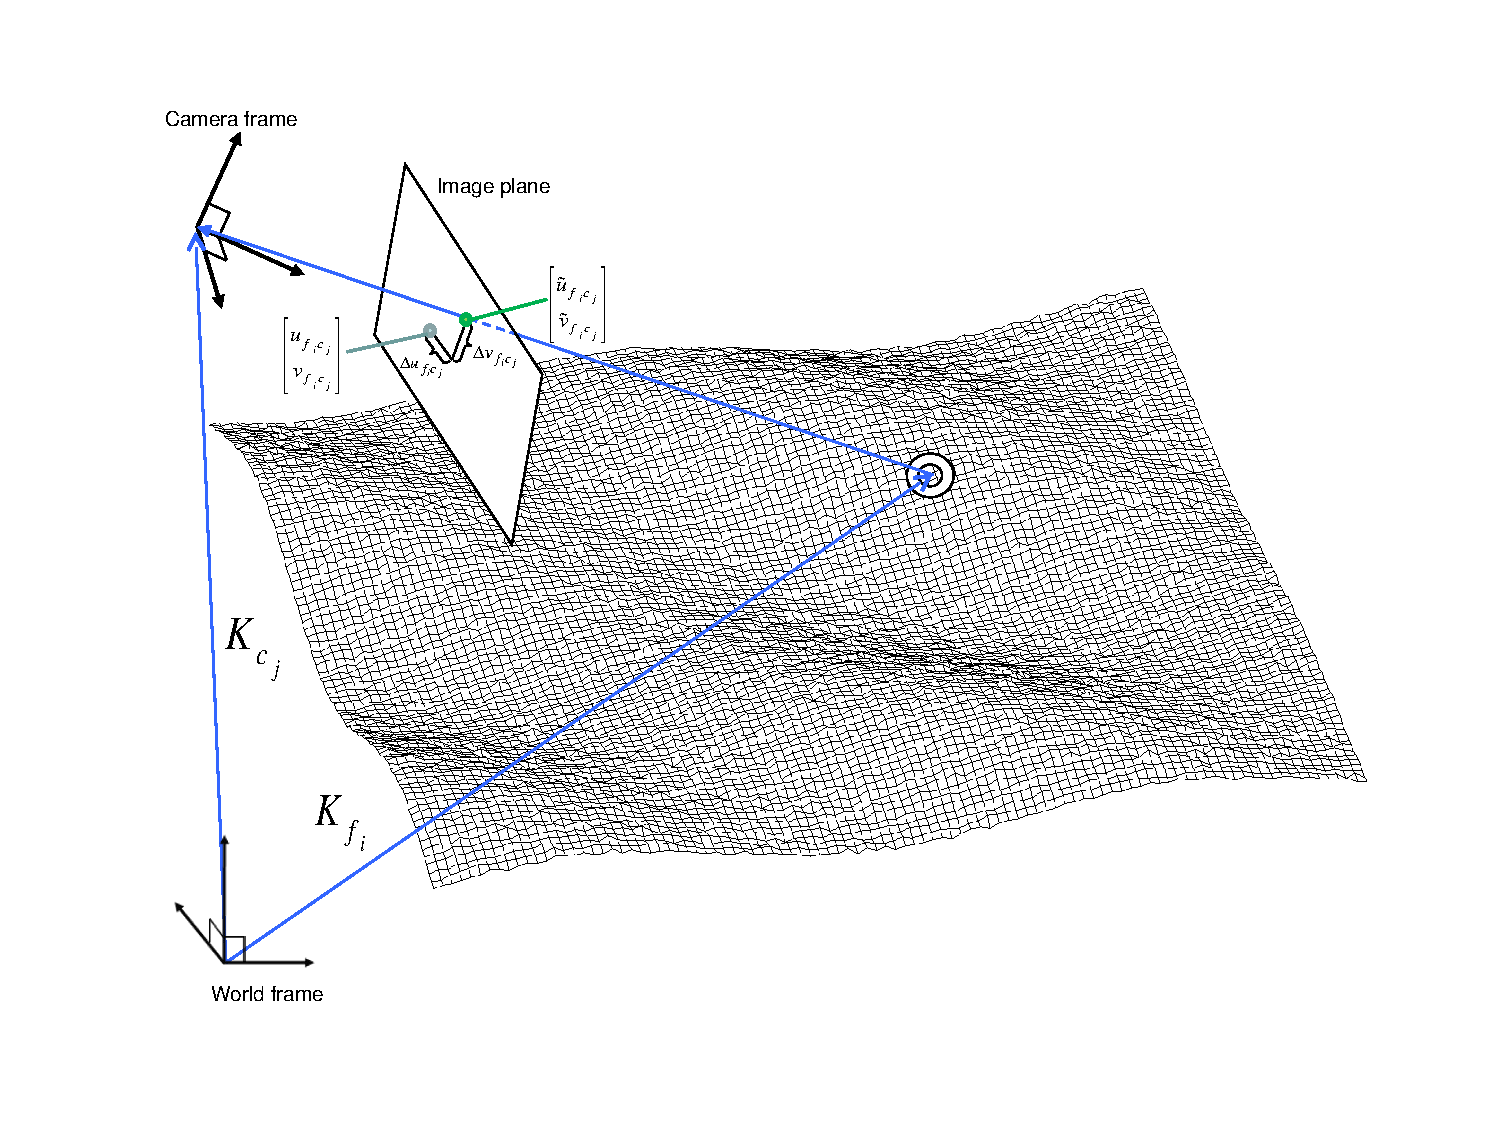
\includegraphics[trim=20mm 20mm 20mm 15mm,clip,width=6in]{images/ba_feature_observation.pdf}
  \end{center}
  \caption{ A feature observation in bundle adjustment, from \citet{moore09} }
  \label{fig:ba_feature}
\end{figure}

Bundle Adjustment in \ac{ISIS} is performed with the \texttt{jigsaw}
executable. It generally follows the method described
in~\cite{triggs00} and determines the best camera parameters that
minimize the projection error given by ${\bf \epsilon} =
\sum_k\sum_j(I_k-I(C_j, X_k))^2$ where $I_k$ are the tie points on the
image plane, $C_j$ are the camera parameters, and $X_k$ are the 3D
positions associated with features $I_k$. $I(C_j, X_k)$ is an image
formation model (i.e. forward projection) for a given camera and 3D
point. To recap, it projects the 3D point, $X_k$, into the camera with
parameters $C_j$. This produces a predicted image location for the 3D
point that is compared against the observed location, $I_k$. It then
reduces this error with the Levenberg-Marquardt algorithm (LMA). Speed
is improved by using sparse methods as described in \citet{hartley04},
\citet{konolige:sparsesparse}, and \citet{cholmod}.

Even though the arithmetic for bundle adjustment sounds clever, there
are faults with the base implementation. Imagine a case where all
cameras and 3D points were collapsed into a single point. If you
evaluate the above cost function, you'll find that the error is indeed
zero. This is not the correct solution if the images were taken
from orbit. Another example is if a translation was applied equally to
all 3D points and camera locations. This again would not affect the
cost function. This fault comes from bundle adjustment's inability to
control the scale and translation of the solution. It will correct the
geometric shape of the problem, yet it cannot guarantee that the solution
will have correct scale and translation.

\ac{ISIS} attempts to fix this problem by adding two additional cost
functions to bundle adjustment. First of which is ${\bf \epsilon} =
\sum_j(C_j^{initial}-C_j)^2$. This constrains camera parameters to
stay relatively close to their initial values. Second, a small handful
of 3D ground control points can be chosen by hand and added to the
error metric as ${\bf \epsilon} = \sum_k(X_k^{gcp}-X_k)^2$ to
constrain these points to known locations in the planetary coordinate
frame. A physical example of a ground control point could be the
location of a lander that has a well known location. \acp{GCP} could also be
hand-picked points against a highly regarded and prior existing map
such as the THEMIS Global Mosaic or the LRO-WAC Global Mosaic.

Like other iterative optimization methods, there are several
conditions that will cause bundle adjustment to terminate. When
updates to parameters become insignificantly small or when the error,
${\bf \epsilon}$, becomes insignificantly small, then the algorithm
has converged and the result is most likely as good as it will get.
However, the algorithm will also terminate when the number of
iterations becomes too large in which case bundle adjustment may or
may not have finished refining the parameters of the cameras.

\subsection{Tutorial: Processing Mars Orbital Camera Imagery}
\label{sec:ba_example}

This tutorial for ISIS's bundle adjustment tools is taken from
\cite{lunokhod:controlnetwork} and \cite{lunokhod:gcp}. These tools
are not a product of NASA nor the authors of Stereo Pipeline. They
were created by USGS and their documentation is available at
\cite{isis:documentation}.

What follows is an example of bundle adjustment using two \ac{MOC}
images of Hrad Vallis. We use images E02/01461 and M01/00115, the same
as used in Chapter~\ref{ch:moc_tutorial}. These images are available from
NASA's \ac{PDS} (the \ac{ISIS} \texttt{mocproc} program will operate
on either the IMQ or IMG format files, we use the \texttt{.imq} below
in the example).  For reference, the following \ac{ISIS} commands are
how to convert the \ac{MOC} images to \ac{ISIS} cubes.

\begin{verbatim}
  ISIS 3> mocproc from=e0201461.imq to=e0201461.cub mapping=no
  ISIS 3> mocproc from=m0100115.imq to=m0100115.cub mapping=no
\end{verbatim}

Note that the resulting images are not map-projected. Bundle
adjustment requires the ability to project arbitrary 3D points into
the camera frame. The process of map-projecting an image dissociates
the camera model from the image. Map-projecting can be perceived as
the generation of a new infinitely large camera sensor that may be
parallel to the surface, a conic shape, or something more
complex. That makes it extremely hard to project a random point into
the camera's original model. The math would follow the transformation
from projection into the camera frame, then projected back down to
surface that ISIS uses, then finally up into the infinitely large
sensor. \texttt{Jigsaw} does not support this and thus does not
operate on map-projected imagery.

Before we can dive into creating our tie-point measurements we must
finish prepping these images. The following commands will add a vector
layer to the cube file that describes its outline on the globe. It
will also create a data file that describes the overlapping sections
between files.

\begin{verbatim}
  ISIS 3> footprintinit from=e0201461.cub
  ISIS 3> footprintinit from=m0100115.cub
  ISIS 3> echo *cub |  xargs -n1 echo > cube.lis
  ISIS 3> findimageoverlaps from=cube.lis overlaplist=overlap.lis
\end{verbatim}

At this point, we are ready to start generating our measurements. This
is a three step process that requires defining a geographic pattern
for the layout of the points on the groups, an automatic registration
pass, and finally a manual clean up of all measurements. Creating the
ground pattern of measurements is performed with \texttt{autoseed}. It
requires a settings file that defines the spacing in meters between
measurements. For this example, write the following text into a
\textit{autoseed.def} file.

\begin{verbatim}
  Group = PolygonSeederAlgorithm
        Name = Grid
        MinimumThickness = 0.01
        MinimumArea = 1
        XSpacing = 1000
        YSpacing = 2000
  End_Group
\end{verbatim}

The minimum thickness defines the minimum ratio between the sides of
the region that can have points applied to it. A choice of 1 would
define a square and anything less defines thinner and thinner
rectangles. The minimum area argument defines the minimum square
meters that must be in an overlap region. The last two are the spacing
in meters between control points. Those values were specifically
chosen for this pair so that about 30 measurements would be produced
from \texttt{autoseed}. Having more control points just makes for more
work later on in this process. Run \texttt{autoseed} with the
following instruction.

\begin{figure}[ht]
  \centering
  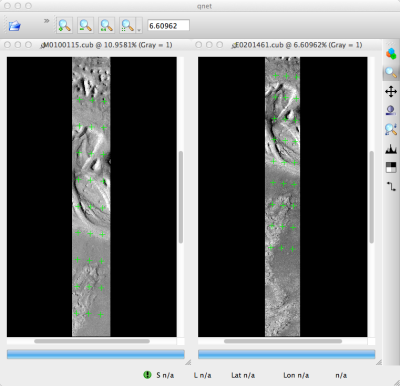
\includegraphics[width=5in]{images/qnet/Qnet_AfterAutoseed_400px.png}
  \caption{A visualization of the features laid out by
    \texttt{autoseed} in \texttt{qnet}. Note that the marks do not
    cover the same features between images. This is due to the poor
    initial spice data for MOC imagery.}
  \label{fig:after_autoseed}
\end{figure}

\begin{verbatim}
  ISIS 3> autoseed fromlist=cube.lis overlaplist=overlap.lis    \
            onet=control.net deffile=autoseed.def networkid=moc \
            pointid=???? description=hrad_vallis
\end{verbatim}

The next step is to perform auto registration of these features
between the two images using \texttt{pointreg}. This program also
requires a settings file that describes how to do the automatic
search. Copy the text box below into a \textit{autoRegTemplate.def}
file.

\begin{verbatim}
   Object = AutoRegistration
    Group = Algorithm
      Name         = MaximumCorrelation
      Tolerance    = 0.7
    EndGroup

    Group = PatternChip
      Samples = 21
      Lines   = 21
      MinimumZScore = 1.5
      ValidPercent = 80
    EndGroup

    Group = SearchChip
      Samples = 75
      Lines   = 1000
    EndGroup
  EndObject
\end{verbatim}

The search chip defines the search range for which \texttt{pointreg}
will look for matching imagery. The pattern chip is simply the kernel
size of the matching template. The search range is specific for this
image pair. The control network result after \texttt{autoseed} had a
large vertical offset in the ball park of 500 px. The large
misalignment dictated the need for the large search in the lines
direction. Use \texttt{qnet} to get an idea for what the pixel shifts
look like in your stereo pair to help you decide on a search range. In
this example, only one measurement failed to match automatically. Here
are the arguments to use in this example of \texttt{pointreg}.

\begin{verbatim}
  ISIS 3> pointreg fromlist=cube.lis cnet=control.net             \
             onet=control_pointreg.net deffile=autoRegTemplate.def
\end{verbatim}

The third step is to manually edit the control and verify the
measurements in \texttt{qnet}. Type \texttt{qnet} in the terminal and
then open \textit{cube.lis} and lastly
\textit{control\_pointreg.net}. From the Control Network Navigator
window, click on the first point listed as \textit{0001}. That opens a
third window called the Qnet Tool. That window will allow you to play
a flip animation that shows alignment of the feature between the two
images. Correcting a measurement is performed by left clicking in the
right image, then clicking \textit{Save Measure}, and finally
finishing by clicking \textit{Save Point}.

In this tutorial, measurement \textit{0025} ended up being
incorrect. Your number may vary if you used different settings than
the above or if MOC spice data has improved since this writing. When
finished, go back to the main Qnet window. Save the final control
network as \textit{control\_qnet.net} by clicking on \textit{File},
and then \textit{Save As}.

\begin{figure}[ht]
  \centering
  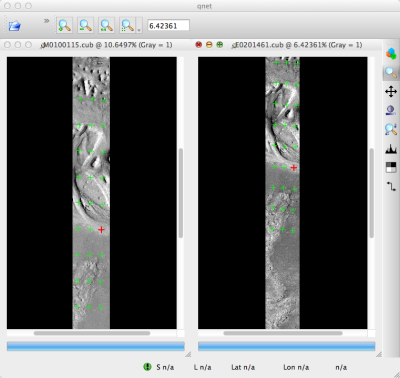
\includegraphics[width=5in]{images/qnet/Qnet_AfterQnetManual_400px.png}
  \caption{A visualization of the features after manual editing in
    \texttt{qnet}. Note that the marks now appear in the same location
    between images.}
  \label{fig:after_manual}
\end{figure}

Once the control network is finished, it is finally time to start
bundle adjustment. Here's what the call to \texttt{jigsaw} looks like:

\begin{verbatim}
  ISIS 3> jigsaw fromlist=cube.lis update=yes twist=no radius=yes \
             cnet=control_qnet.net onet=control_ba.net
\end{verbatim}

The update option defines that we would like to update the camera
pointing, if our bundle adjustment converges. The \textit{twist=no}
says to not solve for the camera rotation about the camera bore. That
property is usually very well known as it is critical for integrating
an image with a line-scan camera. The \textit{radius=yes} means that
the radius of the 3D features can be solved for. Using no will force
the points to use height values from another source, usually LOLA or
MOLA.

The above command will spew out a bunch of diagnostic information from
every iteration of the optimization algorithm. The most important
feature to look at is the \textit{sigma0} value. It represents the mean of
pixel errors in the control network. In our run, the initial error was
1065 px and the final solution had an error of 1.1 px.

Producing a DEM using the newly created camera corrections is the same
as covered in the Tutorial on page \pageref{ch:moc_tutorial}. When using
\texttt{jigsaw}, it modifies a copy of the spice data that is stored
internally to the cube file. Thus when we want to create a DEM using
the correct camera geometry, no extra information needs to be given to
\texttt{stereo} since it is already contained in the file. In the
event a mistake has been made, \texttt{spiceinit} will overwrite the
spice data inside a cube file and provide the original uncorrected
camera pointing.

\begin{verbatim}
  ISIS 3> stereo E0201461.cub M0100115.cub bundled/bundled
\end{verbatim}

%% \subsection{Processing with Ground Control Points}

%% Ground control point files describe a single point in the world
%% that is seen by 1 or more cameras. How they are measured in the
%% first place is up to the user. We use a manual process of comparing
%% each image to a respected map-projected image and then recording
%% the latitude, longitude, and altitude of the point(s). The maps to
%% register against can be anything, but it is recommended to register
%% against a product with a high amount of cartographic stability and
%% accuracy.  For terrestrial work, we would use a \ac{USGS} product
%% that can provide imagery that is registered to LIDAR height
%% measurements.

%% Unlike match files, ground control points must specifically be given
%% to \texttt{isis\_adjust} from the command line, but in no particular
%% order. Ground control point files are written with the extension
%% \texttt{.gcp}. Below is an example of a ground control point file that
%% was created to control a series of Apollo Metric Camera images from
%% several Apollo 15 orbits.

%% \begin{verbatim}
%%     -52.8452 27.2561 1735999 300 300 500
%%     sub4-AS15-M-2086.cub     210.9   3565.0
%%     sub4-AS15-M-2087.cub     1476.9  3579.0
%%     sub4-AS15-M-2088.cub     2798.9  3586.8
%%     sub4-AS15-M-2089.cub     4133.5  3588.6
%%     sub4-AS15-M-2344.cub     906.9   3874.8
%%     sub4-AS15-M-2345.cub     2204.2  3913.9
%%     sub4-AS15-M-2482.cub     939.8   4348.0
%%     sub4-AS15-M-2483.cub     2282.0  4340.7
%%     sub4-AS15-M-2484.cub     3642.1  4330.9
%% \end{verbatim}

%% The first line of a \texttt{.gcp} file is like a header line and
%% is different from the remaining lines.  The first line defines the
%% world location of the ground control point, and the rest of the
%% lines define the image locations of the ground control points. Here
%% are what the columns mean for the first line.

%% \begin{myindentpar}{2cm}
%% \begin{description}
%%   \item[Column 1:] Longitude in degrees
%%   \item[Column 2:] Latitude in degrees
%%   \item[Column 3:] Radius in meters
%%   \item[Column 4:] Sigma (or uncertainty) in meters for Local X axis
%%   \item[Column 5:] Sigma (or uncertainty) in meters for Local Y axis
%%   \item[Column 6:] Sigma (or uncertainty) in meters for Local Z axis
%% \end{description}
%% \end{myindentpar}

%% The other lines describe where this \ac{GCP} is found in each image:

%% \begin{myindentpar}{2cm}
%% \begin{description}
%%   \item[Column 1:] Image name
%%   \item[Column 2:] Sample (X) image measurement
%%   \item[Column 3:] Line (Y) image measurement
%% \end{description}
%% \end{myindentpar}

%% Make a {\tt .gcp} file for every ground control point, then be sure
%% to feed them as an input to {\tt isis\_adjust}. Remember that you
%% can scale the sigma of all ground control points by using the {\tt
%% -\/-gcp-scalar} flag. This can save time by allowing you to make
%% adjustments without needing to edit all of the files individually.
